%% PLACE CONTACT INFORMATION HERE


\chapter[Short title]{Much more explanatory title i.e. the long title}\label{chap:LABELTITLE4}
\footnote{If this chapter is based on published work, explain that in this footnote} 

\begin{refsection}

\abstract{
Abstract of this chapter
}

\newpage	
\section{Section 1}

Write about stuff, and stuff and more stuff. Then perhaps show a figure, which you can reference with (Figure \ref{fig:LABELFORFIG4_1}).

\begin{figure}
\begin{center}
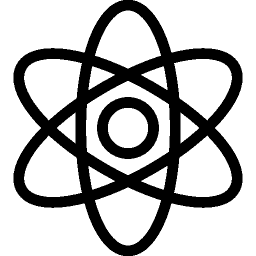
\includegraphics[width=0.7\columnwidth]{./C4_Topic3/figure_1/fig1.png}
\caption{\label{fig:LABELFORFIG4_1} This is where you write the caption belonging to this figure}
\end{center}
\end{figure}


%\newpage
\section{Section 2}

Perhaps we also cite some literature \cite{Marion1995}. This bibliography is a seperate file and specific to the chapter by the way  \cite{Marion1995, rezakhaniha2012}.

\subsection{subsection 1}
We can also use subsections 


\subsection{subsection 2}
Another figure example.

\begin{figure}
\begin{center}
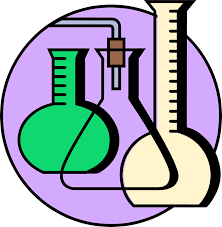
\includegraphics[width=0.7\columnwidth]{./C4_Topic3/figure_2/fig2.png}
\caption{\label{fig:LABELFORFIG4_2} This is where you write the caption belonging to this figure}
\end{center}
\end{figure}


blablabla (Figure \ref{fig:LABELFORFIG4_2}). Now let's do a table (Table \ref{tab:LABELFORTBL3_1})

\begin{table}[H]
\centering
\begin{tabular}{l c c | c c}
 	& 	\multicolumn{2}{c}{Overarch1}   		& \multicolumn{2}{c}{Overarch2} \\
 	& A & B 	& C & D \\
\cline{2-5}
BLA & 1 & 2 & 3 & 4 \\
k (nN/$\upmu$m) & 5 & 6 & 7 & 8 \\
\cline{2-5}
\end{tabular}

\caption{\label{tab:LABELFORTBL4_1}This is where you write the caption belonging to this table}
\end{table}

\newpage
\printbibliography[title={Bibliography}]
\end{refsection}

